% !TEX program = xelatex
% 컴파일: xelatex promotion_targeting_policy_learning_whitepaper.tex (kotex + Apple SD Gothic Neo)
\documentclass[11pt]{article}

\usepackage{kotex}
\setmainhangulfont{Apple SD Gothic Neo}
\setsanshangulfont{Apple SD Gothic Neo}

\usepackage{amsmath}
\usepackage{amssymb}
\usepackage{graphicx}
\usepackage{booktabs}
\usepackage{xcolor}
\usepackage{titlesec}
\usepackage{caption}
\usepackage{enumitem}
\usepackage{fancyhdr}
\usepackage[section]{placeins}
\usepackage[a4paper, top=2.6cm, bottom=2.6cm, left=2.8cm, right=2.8cm]{geometry}
\usepackage{hyperref}

\graphicspath{{../figures/}}

% ----- 브랜드 색상 -----
\definecolor{brand}{RGB}{140,22,22}      % 딥 레드 (컨설팅 리포트 톤)
\definecolor{ink}{RGB}{40,40,40}
\definecolor{rulegray}{RGB}{200,200,200}

\hypersetup{
  colorlinks=true, linkcolor=brand, urlcolor=brand, citecolor=brand,
  pdftitle={누구에게 어떤 프로모션을 제공해야 할까},
  pdfauthor={조해창}
}

% ----- 섹션 스타일 -----
\titleformat{\section}{\sffamily\Large\bfseries\color{brand}}{\thesection.}{0.5em}{}
\titleformat{\subsection}{\sffamily\large\bfseries\color{ink}}{\thesubsection}{0.5em}{}
\titlespacing*{\section}{0pt}{1.6em}{0.7em}

% ----- 캡션 스타일 -----
\captionsetup{font=small, labelfont={bf,color=brand}, labelsep=period, skip=6pt}
\renewcommand{\tablename}{표}
\renewcommand{\figurename}{그림}

% ----- 머리말/꼬리말 -----
\pagestyle{fancy}
\fancyhf{}
\renewcommand{\headrulewidth}{0pt}
\renewcommand{\footrulewidth}{0.4pt}
\renewcommand{\footrule}{\hbox to\headwidth{\color{rulegray}\leaders\hrule height \footrulewidth\hfill}}
\fancyfoot[L]{\footnotesize\color{brand} 누구에게 어떤 프로모션을 제공해야 할까 · 정책학습 기반 타겟팅}
\fancyfoot[R]{\footnotesize\color{brand}\thepage}

\setlength{\parskip}{0.6em}
\setlength{\parindent}{0pt}
\renewcommand{\arraystretch}{1.25}

% 핵심 수치 강조용
\newcommand{\kpi}[1]{{\color{brand}\bfseries #1}}

\begin{document}

% =================================================== 표지
\thispagestyle{empty}
\vspace*{1.2cm}
{\sffamily\bfseries\color{brand}\large CAUSAL INFERENCE PORTFOLIO}
\vskip 2pt
{\color{rulegray}\hrule height 1.2pt}

\vspace{4.5cm}
{\sffamily\bfseries\fontsize{30}{36}\selectfont 누구에게 어떤 프로모션을\\[4pt] 제공해야 할까?\par}
\vspace{0.8cm}
{\sffamily\Large\color{ink} 예산 제약 하의 정책학습(Policy Learning) 기반 프로모션 타겟팅\par}

\vspace{3.2cm}
{\sffamily\large\bfseries\color{brand} 데이터 분석 포트폴리오\par}

\vfill
{\footnotesize\color{ink}
\textbf{조해창} \quad
GitHub: \href{https://github.com/Funbucket}{github.com/Funbucket} \quad
LinkedIn: \href{https://www.linkedin.com/in/hae-chang-cho/}{hae-chang-cho}\par
\vskip 4pt
관찰 데이터 · 다중 처치 · Doubly Robust(AIPW) · econml DRLearner/DRPolicyTree/DRPolicyForest
}
\newpage

% =================================================== 요약
\section*{\sffamily\color{brand} 요약 (Executive Summary)}
\addcontentsline{toc}{section}{요약}

\textbf{문제.} 한 소프트웨어 회사는 고객에게 \emph{기술지원}과 \emph{할인} 두 가지 프로모션을 제공할 수 있다(두 개입의 조합으로 총 네 가지 처치). 예산은 제한되어 있고, 프로모션 효과는 고객마다 다르다. 따라서 핵심 질문은 다음과 같다: ``제한된 예산 안에서 누구에게 어떤 프로모션을 제공해야 전체 순이익이 가장 커질까?''

\textbf{접근.} 약 2{,}000곳의 관찰 데이터에 정책학습(policy learning)을 적용했다. (1)~처치 효과의 이질성을 진단하고, (2)~관찰 데이터의 인과 식별 가정을 점검한 뒤, (3)~세 가지 정책(DRLearner plug-in · DRPolicyTree · DRPolicyForest)을 학습하고, (4)~학습/평가 데이터를 분리해 AIPW(doubly robust) score로 정책 가치를 비교했으며, (5)~예산 제약 하의 효율은 비용 곡선(cost curve)으로 평가했다.

\textbf{핵심 결과.}

\begin{table}[h]
\centering
\small
\begin{tabular}{lrr}
\toprule
정책 & 고객사당 평균 순이익 & 처치 없음 대비 \\
\midrule
처치 없음 (all none) & \$7{,}249 & --- \\
최선의 단일 처치 (전원 기술지원) & \$10{,}527 & +45\% \\
\textbf{고객별 타겟팅 (DRLearner plug-in)} & \kpi{\$11{,}798} & \kpi{+63\%} \\
\bottomrule
\end{tabular}
\end{table}

\begin{itemize}[leftmargin=1.4em, itemsep=2pt]
  \item 고객별 타겟팅 정책은 가장 좋은 단일 처치 정책보다 약 12\%, 처치 없음 대비 약 63\% 높은 순이익을 냈다.
  \item 처치 배정을 좌우한 핵심 요인은 직원 수(42\%)와 고객 규모(38\%)였다. 규모가 큰 고객에게는 \emph{기술지원+할인}을, 그 외 고객에게는 주로 \emph{기술지원}을 배정했다.
  \item 예산 수준에 따라 최적 정책이 달랐다. 총 예산 \$3.9M 이하에서는 \emph{전원 기술지원}이 가장 효율적이지만, 그 이상에서는 학습 정책이 더 높은 순이익을 냈다.
\end{itemize}

\textbf{핵심 제안.} 모두에게 동일한 프로모션을 적용하기보다, 고객 규모·직원 수에 기반한 타겟팅 규칙을 적용하길 제안한다. 성능이 최우선이면 plug-in/forest 정책을, 설명·운영 안정성이 중요하면 해석 가능한 depth=2 트리 정책을 권한다.

\newpage

% =================================================== 1. 비즈니스 문제
\section{비즈니스 문제}

인과추론의 많은 문제는 평균 처치 효과(ATE)에 집중한다. ``프로모션을 진행할 것인가, 하지 않을 것인가?''라는 질문은 \emph{모든} 고객에게 동일한 프로모션을 제공하는 정책과 아무에게도 제공하지 않는 정책을 비교하는 문제다.

하지만 예산이 제한되어 있고 그 안에서 최대 효과를 내야 한다면 이야기가 달라진다. 프로모션 효과가 고객마다 다르다면, 모두에게 동일하게 제공하는 전략이 최선이 아닐 수 있다.

\begin{itemize}[leftmargin=1.4em, itemsep=2pt]
  \item 마케팅 유무와 상관없이 어차피 구매하거나(\emph{always-converters}), 반대로 아무리 혜택을 줘도 사지 않을 고객(\emph{lost causes})에게 불필요한 예산을 낭비하게 된다.
  \item 마케팅에 부정적으로 반응하는 고객(\emph{sleeping dogs}) 때문에 오히려 손실이 발생하며,
  \item 정작 효과가 클 고객(\emph{high-responders})을 우선순위에 두지 못해 잠재 매출을 놓친다.
\end{itemize}

따라서 이 분석이 답하려는 질문은 \emph{``어떤 고객을 대상으로 해야 순이익이 가장 커질까?''}이다. 가능한 처치 규칙들을 탐색해 전체 평균 순수익을 근사적으로 최대화하는 문제, 즉 ``누구를 처치해야 하는가?''에 답하는 문제를 정책학습(policy learning)이라고 부른다.

이 분석은 다음 다섯 가지 질문으로 구성된다.

\begin{description}[leftmargin=2.4em, itemsep=2pt]
  \item[Q1.] 프로모션 효과는 정말 고객마다 다른가? (이질성 진단)
  \item[Q2.] 관찰 데이터로 인과 효과를 신뢰할 수 있는가? (식별 가정)
  \item[Q3.] 누구에게 무엇을 배정해야 하는가? (정책학습)
  \item[Q4.] 학습한 정책이 정말 더 나은가? (정책 평가)
  \item[Q5.] 예산이 제한되면 어떤 정책이 유리한가? (예산 제약)
\end{description}

% =================================================== 2. 데이터
\section{데이터와 처치 정의}

무작위 실험(RCT)이 가장 이상적이지만, 실제 비즈니스 환경에서는 비용 문제, 영업 전략, 대형 고객을 놓칠 위험 등으로 무작위 실험을 수행하기 어렵다. 따라서 이번 데이터는 무작위 실험 데이터가 아닌 관찰 데이터이며, 약 2{,}000곳의 고객 정보로 구성된다(고객 특성 8종, 개입 2종, 결과 1종).

\texttt{Tech Support}와 \texttt{Discount}는 모두 개입이므로, 이를 조합해 네 가지 처치로 정의한다($A_i \in \{0,1,2,3\}$).

\begin{table}[h]
\centering
\small
\caption{네 가지 처치 정의}
\begin{tabular}{cll}
\toprule
$A_i$ & 이름 & 의미 \\
\midrule
0 & none & 아무 개입도 제공하지 않음 \\
1 & tech\_support\_only & 기술지원만 제공 \\
2 & discount\_only & 할인만 제공 \\
3 & discount\_plus\_support & 기술지원과 할인을 모두 제공 \\
\bottomrule
\end{tabular}
\end{table}

\subsection{비용 설정}

수익 극대화를 위해서는 매출과 함께 비용도 고려해야 한다. 동일한 프로모션이라도 고객 특성에 따라 비용이 달라질 수 있다. 이 데이터에는 실제 비용 정보가 없으므로, 기술지원 비용은 직원 수가 많을수록, 할인 비용은 고객 규모가 클수록 증가하도록 시뮬레이션한다. 비용이 항상 양수이고 일부 고객에서 큰 비용이 발생하는 분포를 반영하기 위해 로그정규분포를 사용한다.

\[
C_i(\text{tech}) \sim \text{LogNormal}(\log C_{\text{tech}} + 0.5\,\tilde{e}_i,\ 0.3), \qquad
C_i(\text{disc}) \sim \text{LogNormal}(\log C_{\text{disc}} + 0.4\,\tilde{s}_i,\ 0.3)
\]

여기서 $\tilde{e}_i$는 표준화된 직원 수, $\tilde{s}_i$는 표준화된 회사 규모다. 고객별 비용을 반영한 최종 순이익(net outcome)은 $Y_i^{net} = Y_i - C_i(A_i)$로 정의한다. 이렇게 하면 이후 AIPW score가 순이익 기준으로 계산되어, 비용을 고려한 정책 최적화와 평가가 가능해진다. 정책 학습과 평가는 train/test를 50:50으로 분리해(각 1{,}000곳) 과대추정을 방지한다.

% =================================================== Q1
\section{Q1. 프로모션 효과는 정말 고객마다 다른가?}

타겟팅이 의미가 있으려면 먼저 처치 효과가 고객마다 다르다는 신호가 있어야 한다. 처치별 표본은 23\,$\sim$\,27\%로 고르게 분포해(표~\ref{tab:summary}) 비교에 안정적이다. 한편 처치별 평균 매출은 처치 없음일 때 6{,}586, 기술지원+할인일 때 26{,}784로, 처치에 따라 4배 이상 차이가 난다.

\begin{table}[h]
\centering
\small
\caption{처치별 표본 수·평균 매출·평균 비용·평균 순이익}
\label{tab:summary}
\begin{tabular}{lrrrr}
\toprule
처치 & 표본 수 & 평균 매출 & 평균 비용 & 평균 순이익 \\
\midrule
none & 517 & 6{,}586 & 0 & 6{,}586 \\
tech\_support\_only & 462 & 15{,}104 & 5{,}038 & 10{,}066 \\
discount\_only & 477 & 12{,}248 & 5{,}182 & 7{,}066 \\
discount\_plus\_support & 544 & 26{,}784 & 12{,}665 & 14{,}119 \\
\bottomrule
\end{tabular}
\end{table}

그러나 이 평균 차이를 그대로 처치 효과로 해석하면 안 된다. 그림~\ref{fig:cov}에서 보듯 처치 그룹별 고객 특성이 다르고(특히 \texttt{Size}, \texttt{IT Spend}), 규모가 큰 고객일수록 더 강한 개입을 받는 경향이 있다. 즉 매출 차이에는 고객 특성의 영향과 실제 처치 효과가 함께 섞여 있다(그림~\ref{fig:rev}).

\begin{figure}[h]
\centering
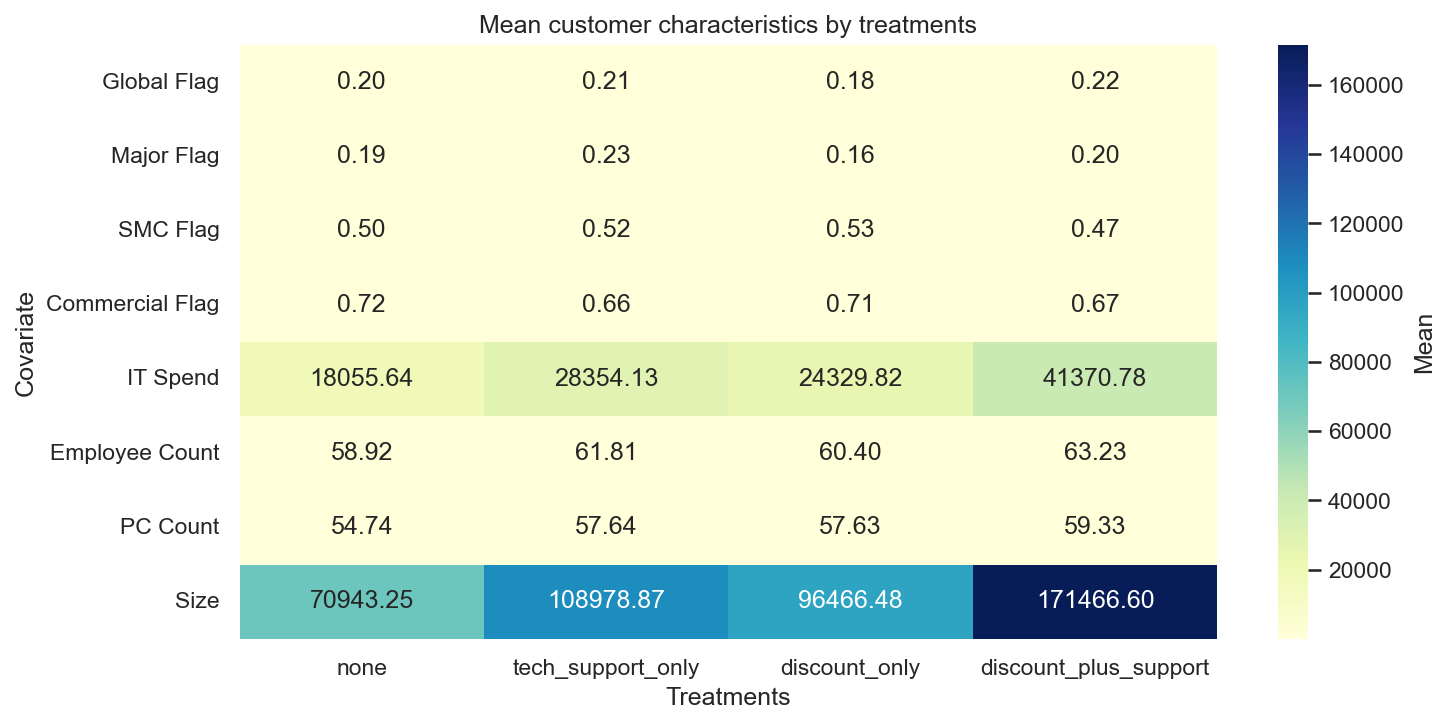
\includegraphics[width=0.82\textwidth]{fig02_covariate_means.png}
\caption{처치별 고객 특성 평균. \texttt{Size}, \texttt{IT Spend}가 처치 그룹마다 다르게 나타나며, 처치 배정이 고객 특성과 얽혀 있음을 보여준다.}
\label{fig:cov}
\end{figure}

\begin{figure}[h]
\centering
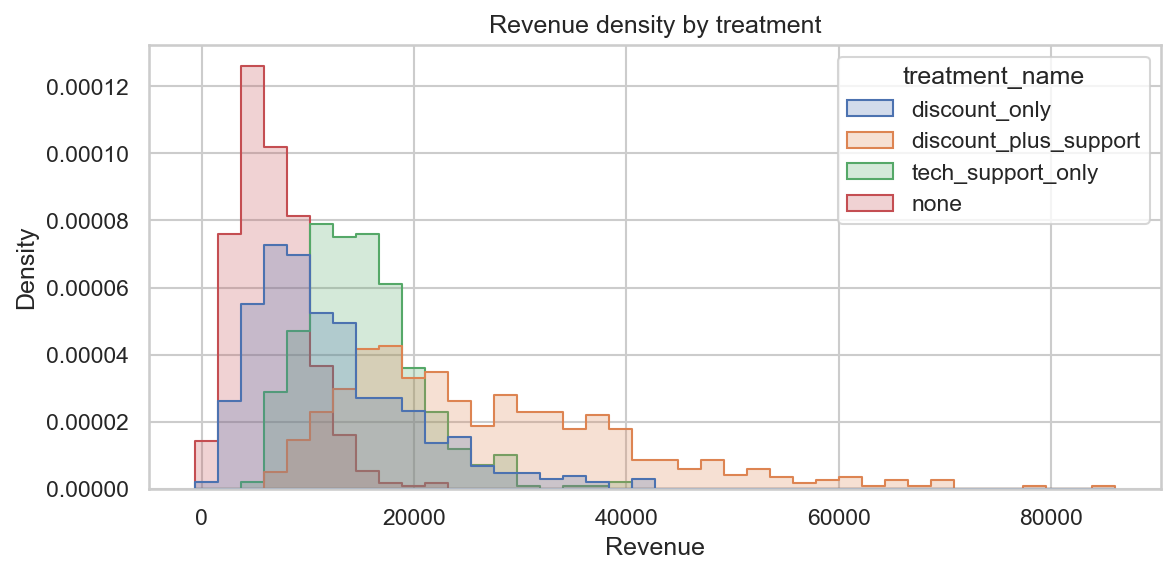
\includegraphics[width=0.72\textwidth]{fig03_revenue_dist.png}
\caption{처치별 Revenue 분포. 규모·분산·이상치가 처치마다 다르다.}
\label{fig:rev}
\end{figure}

\textbf{Q1 요약.} 처치 그룹 간 고객 특성과 결과 분포가 뚜렷이 다르다. 이는 (a)~처치 효과가 고객마다 다를 가능성과 (b)~처치 배정이 고객 특성에 의해 교란되어 있음을 동시에 시사한다. 따라서 단순 평균 비교가 아니라 교란을 보정하는 인과적 접근이 필요하다.

% =================================================== Q2
\section{Q2. 관찰 데이터로 인과 효과를 신뢰할 수 있는가?}

관찰 데이터에서 AIPW 추정이 인과적으로 유효하려면 두 가지 가정이 필요하다.

\textbf{1. Unconfoundedness (비교란성).}\quad
$\{Y_i(0), Y_i(1), Y_i(2), Y_i(3)\} \perp A_i \mid X_i$. 관측된 공변량 $X_i$를 조건부로 했을 때 처치 배정이 잠재 결과와 독립이어야 한다. 즉, 고객 규모·IT 지출·직원 수 등이 처치 배정을 충분히 설명한다고 가정한다.

\textbf{2. Positivity (양수성).}\quad
$P(A_i = a \mid X_i = x) > 0,\ \forall a,\ \forall x$. 모든 고객 특성 범위에서 각 처치가 어느 정도 관측되어야 한다. 이는 propensity score $e_a(x) = P(A_i = a \mid X_i = x)$를 추정해 직접 확인할 수 있다.

\begin{figure}[h]
\centering
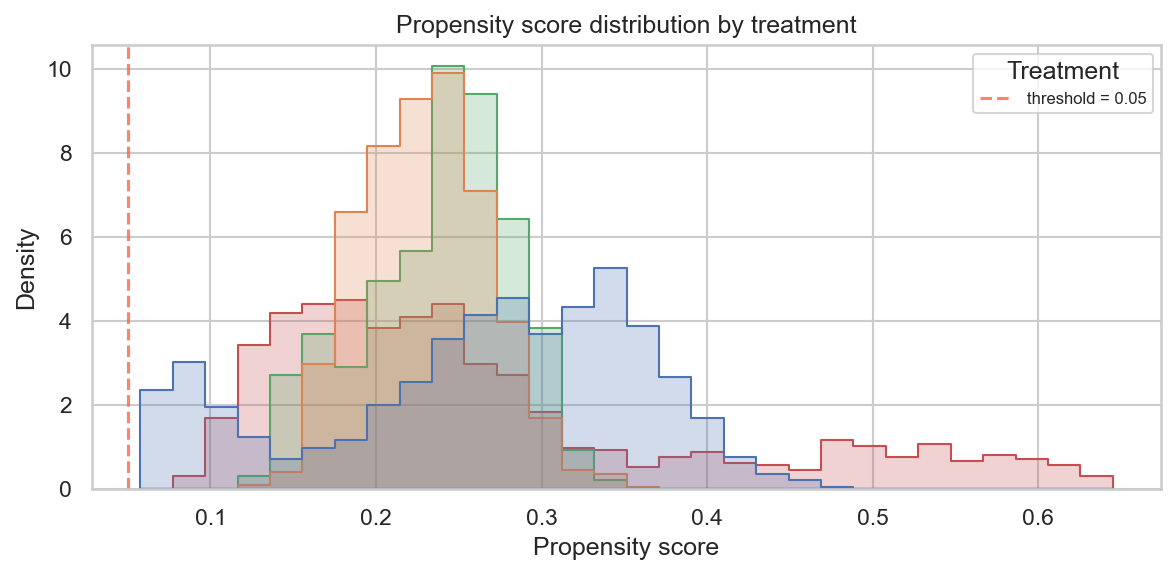
\includegraphics[width=0.72\textwidth]{fig04_propensity.png}
\caption{처치별 propensity score 분포. 네 처치의 분포가 잘 겹치며, $\hat e_a(X_i)$의 최솟값은 약 0.058로 \texttt{0.05} 미만 관측치가 없다.}
\label{fig:prop}
\end{figure}

이 데이터에서 $\hat e_a(X_i)$의 최솟값은 약 0.058이며, \texttt{0.05} 미만 관측치도 없다(그림~\ref{fig:prop}). 즉 극단적으로 작은 propensity score로 일부 관측치에 과도한 가중치가 부여되는 문제는 크지 않다.

\textbf{Q2 요약.} Positivity는 데이터로 확인되어 충족된다. Unconfoundedness는 검정 불가능한 가정이지만, 처치 배정을 설명할 핵심 변수들이 관측되어 있어 합리적인 가정으로 받아들인다. 따라서 이후 분석은 outcome model과 propensity model을 함께 쓰는 doubly robust(AIPW) 추정을 채택한다.

% =================================================== Q3
\section{Q3. 누구에게 무엇을 배정해야 하는가?}

세 가지 정책을 학습해 비교한다.

\begin{itemize}[leftmargin=1.4em, itemsep=2pt]
  \item \textbf{Plug-in Policy (DRLearner):} 고객별 CATE를 추정한 뒤 기대 순이익이 가장 큰 처치를 선택. 유연하지만 CATE 추정 품질에 민감.
  \item \textbf{DRPolicyTree:} AIPW score를 직접 최대화하되 정책을 얕은 의사결정 트리로 제한 $\Rightarrow$ 해석 가능.
  \item \textbf{DRPolicyForest:} AIPW score를 직접 최대화하되 forest 사용 $\Rightarrow$ 분산이 작고 안정적이지만 해석은 어려움.
\end{itemize}

\subsection{Plug-in Policy}
먼저 `처치 없음(none)'을 기준으로 삼아, 각 프로모션이 \emph{처치 없음 대비} 순이익을 얼마나 더 늘리는지(상대효과)를 \texttt{DRLearner}로 추정한다. 즉 $\hat\tau_a(x) = \widehat{\mathbb{E}}[Y^{net}(a) - Y^{net}(0)\mid X=x]$이다. 그런 다음 고객마다 네 선택지의 기대 이득 $[\,0,\ \hat\tau_1(x),\ \hat\tau_2(x),\ \hat\tau_3(x)\,]$를 비교해 가장 큰 값을 주는 처치를 고른다. 첫 항이 0인 이유는 `처치 없음'이 기준이라 자기 자신과의 차이가 0이기 때문이다.
\[
\hat\pi_{\text{plugin}}(x) = \arg\max_{a \in \{0,1,2,3\}} \widehat{\mathbb{E}}[Y^{net}(a) - Y^{net}(0)\mid X=x]
\]
이 정책은 약 50\%에게 기술지원, 37\%에게 기술지원+할인, 약 9\%에게 처치 없음을 배정한다. 기대 순이익이 음수인 일부 고객에게는 처치하지 않는 선택이 나타난다.

\subsection{Policy Tree}
현업에서는 성능뿐 아니라 정책의 설명 가능성도 중요하다. 얕은 의사결정 트리 정책은 (i)~이해관계자 설명, (ii)~공정성 검토, (iii)~운영 안정성 측면에서 유리하다. 이때 정책을 모든 함수가 아니라 제한된 정책 클래스 $\Pi$(얕은 트리) 안에서 탐색한다.
\[
\hat\pi = \arg\max_{\pi \in \Pi} \frac{1}{n}\sum_{i=1}^{n} \widehat\Gamma_{i,\pi(X_i)}
\]

\begin{figure}[h]
\centering
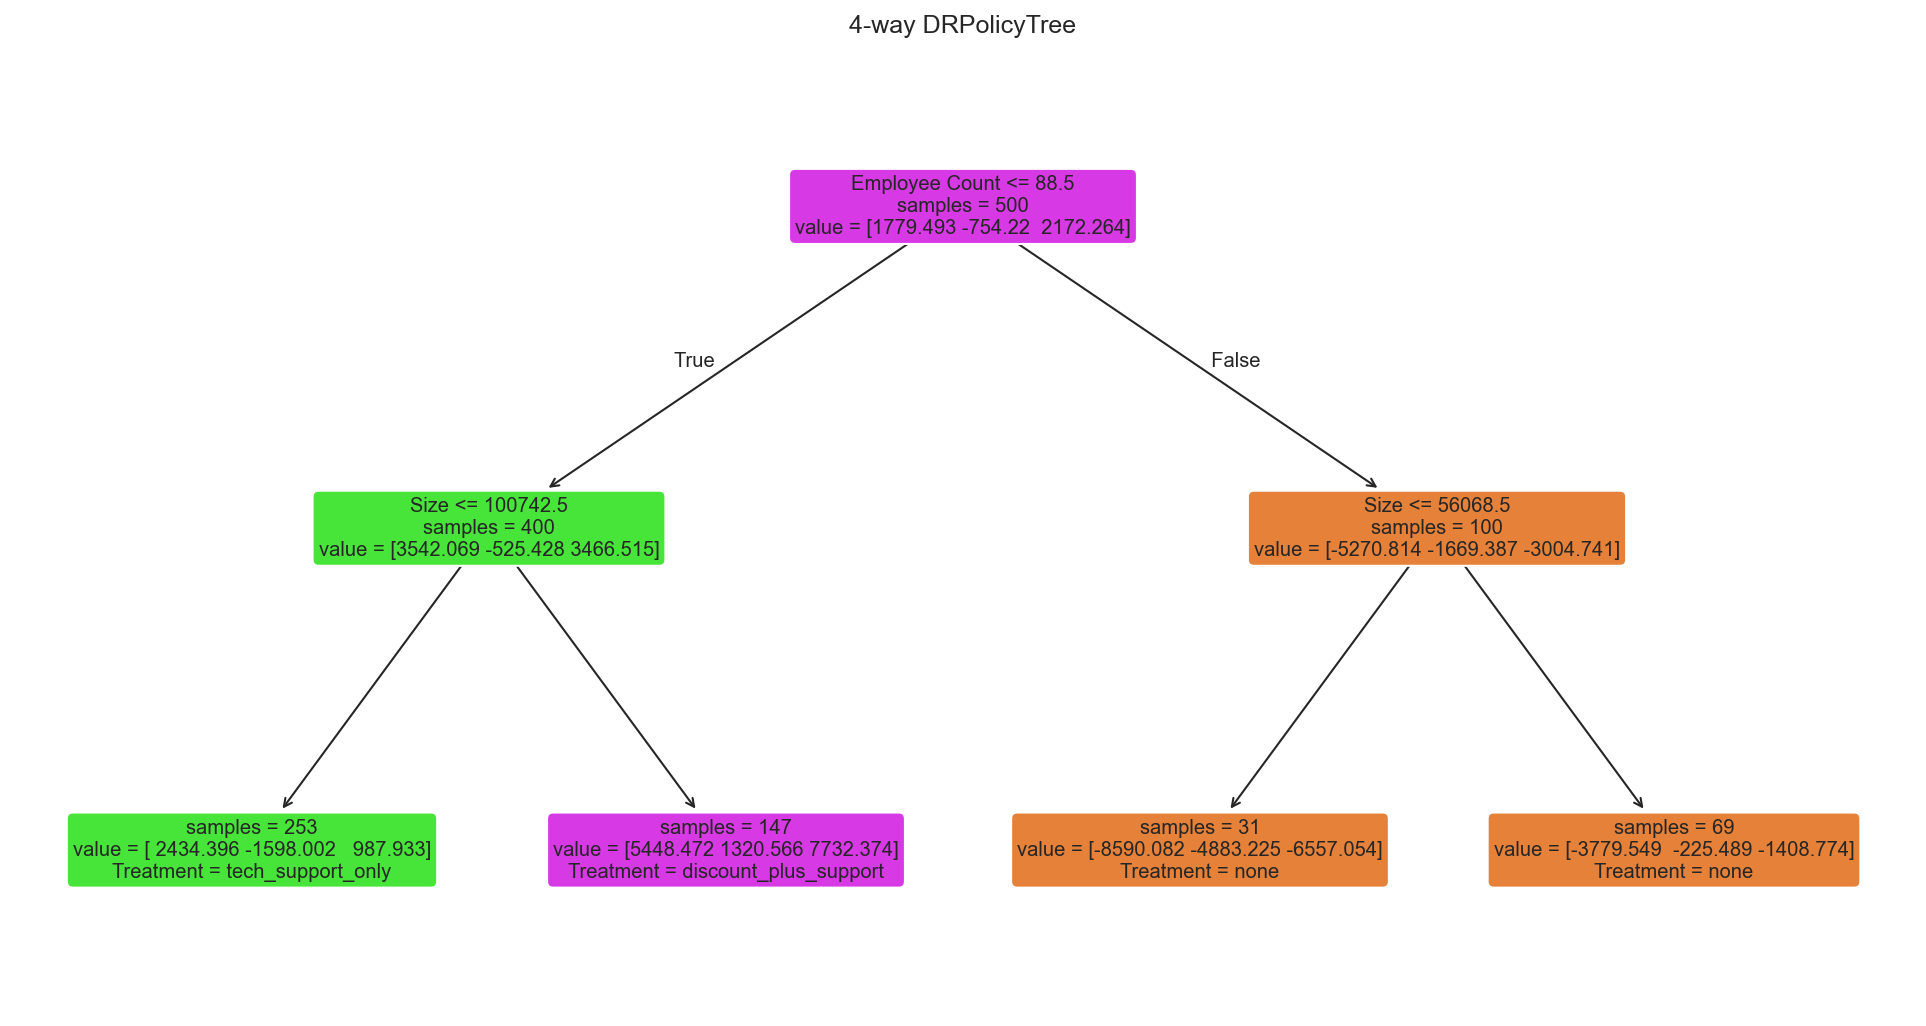
\includegraphics[width=0.95\textwidth]{fig05_policy_tree.png}
\caption{depth=2 DRPolicyTree. 주로 \texttt{Size}를 기준으로 분기한다. 규모가 큰 고객에게는 기술지원+할인을, 그 외에는 주로 기술지원을, 기대 순이익이 낮은 일부(약 20\%)에게는 처치 없음을 배정한다.}
\label{fig:tree}
\end{figure}

\subsection{Policy Forest와 핵심 변수}
Policy Forest는 단일 트리 대신 여러 트리를 평균해 분산이 작고 복잡한 이질성을 안정적으로 학습한다. 단일 규칙으로 해석하기는 어렵지만, 변수 중요도(feature importance)로 어떤 특성이 배정을 주도하는지 파악할 수 있다.

\begin{figure}[h]
\centering
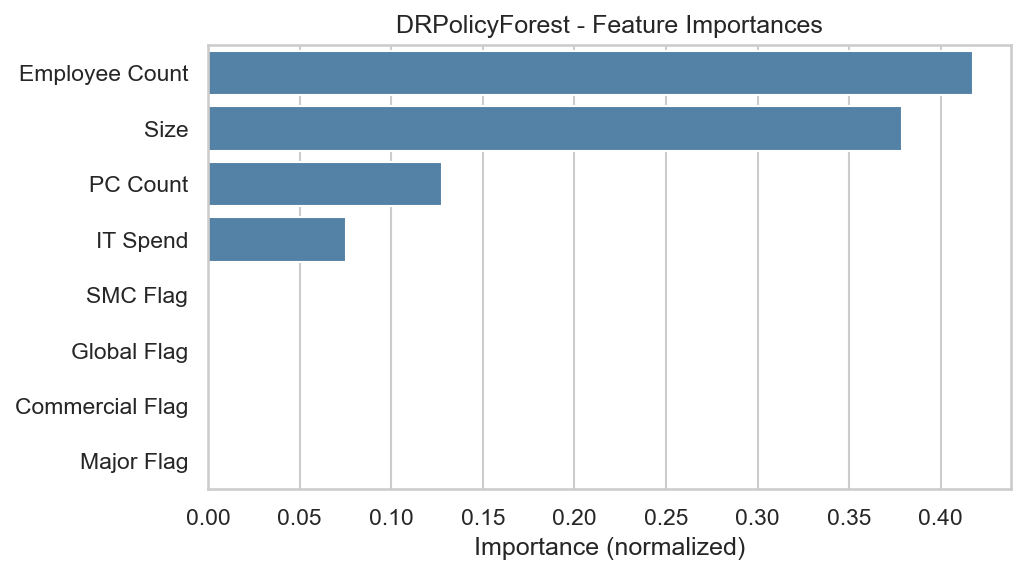
\includegraphics[width=0.7\textwidth]{fig06_feature_importance.png}
\caption{DRPolicyForest 변수 중요도. \texttt{Employee Count}(42\%)와 \texttt{Size}(38\%)가 전체의 약 80\%를 차지한다.}
\label{fig:fi}
\end{figure}

\texttt{Employee Count}(42\%)와 \texttt{Size}(38\%)가 전체 중요도의 약 80\%를 차지하며, 고객 규모와 직원 수가 처치 배정을 주도함을 확인할 수 있다(그림~\ref{fig:fi}). 이는 트리 정책이 \texttt{Size}로 분기한 결과(그림~\ref{fig:tree})와도 일치한다.

\textbf{Q3 요약.} 세 정책 모두 ``규모가 큰 고객 $\to$ 기술지원+할인, 그 외 $\to$ 주로 기술지원, 기대 순이익이 낮은 일부 $\to$ 처치 없음''이라는 일관된 배정 패턴을 학습했다.

% =================================================== Q4
\section{Q4. 학습한 정책이 정말 더 나은가?}

학습한 정책들을 동일한 test set의 AIPW score 기준으로, 모든 고객에게 동일 처치를 적용하는 baseline 정책과 함께 비교한다. AIPW(Augmented Inverse Probability Weighting) score는 다음과 같다.
\[
\hat\Gamma_{i,a} = \hat\mu_a(X_i) + \frac{\mathbf{1}[A_i=a]}{\hat e_a(X_i)}\bigl(Y_i^{net} - \hat\mu_a(X_i)\bigr)
\]
여기서 $\hat\mu_a$는 outcome model, $\hat e_a$는 propensity model의 예측이다. 이 구조 덕분에 둘 중 하나만 올바르게 추정되어도 불편성이 유지된다(doubly robust). 정책 가치의 95\% 신뢰구간은 train set을 100번 재표본추출하고, 매번 정책과 AIPW 평가용 nuisance model을 다시 학습한 뒤 고정된 test set에서 평가하는 학습 포함 bootstrap percentile CI로 계산한다.

\begin{table}[h]
\centering
\small
\caption{정책 가치 비교 (test set AIPW value, 고객사당 평균 순이익, 100회 학습 포함 bootstrap 95\% CI)}
\label{tab:value}
\begin{tabular}{lrr}
\toprule
정책 & AIPW value & 95\% 신뢰구간 \\
\midrule
\textbf{DRLearner plug-in} & \kpi{11{,}798} & [11{,}464,\ 11{,}984] \\
DRPolicyForest & 11{,}619 & [11{,}364,\ 11{,}907] \\
DRPolicyTree (depth=2) & 11{,}149 & [11{,}056,\ 11{,}923] \\
\midrule
all\_tech\_support\_only & 10{,}527 & [10{,}316,\ 10{,}870] \\
all\_discount\_plus\_support & 10{,}137 & [9{,}895,\ 10{,}388] \\
all\_discount\_only & 7{,}545 & [7{,}366,\ 7{,}778] \\
all\_none & 7{,}249 & [7{,}133,\ 7{,}392] \\
\bottomrule
\end{tabular}
\end{table}

\begin{figure}[h]
\centering
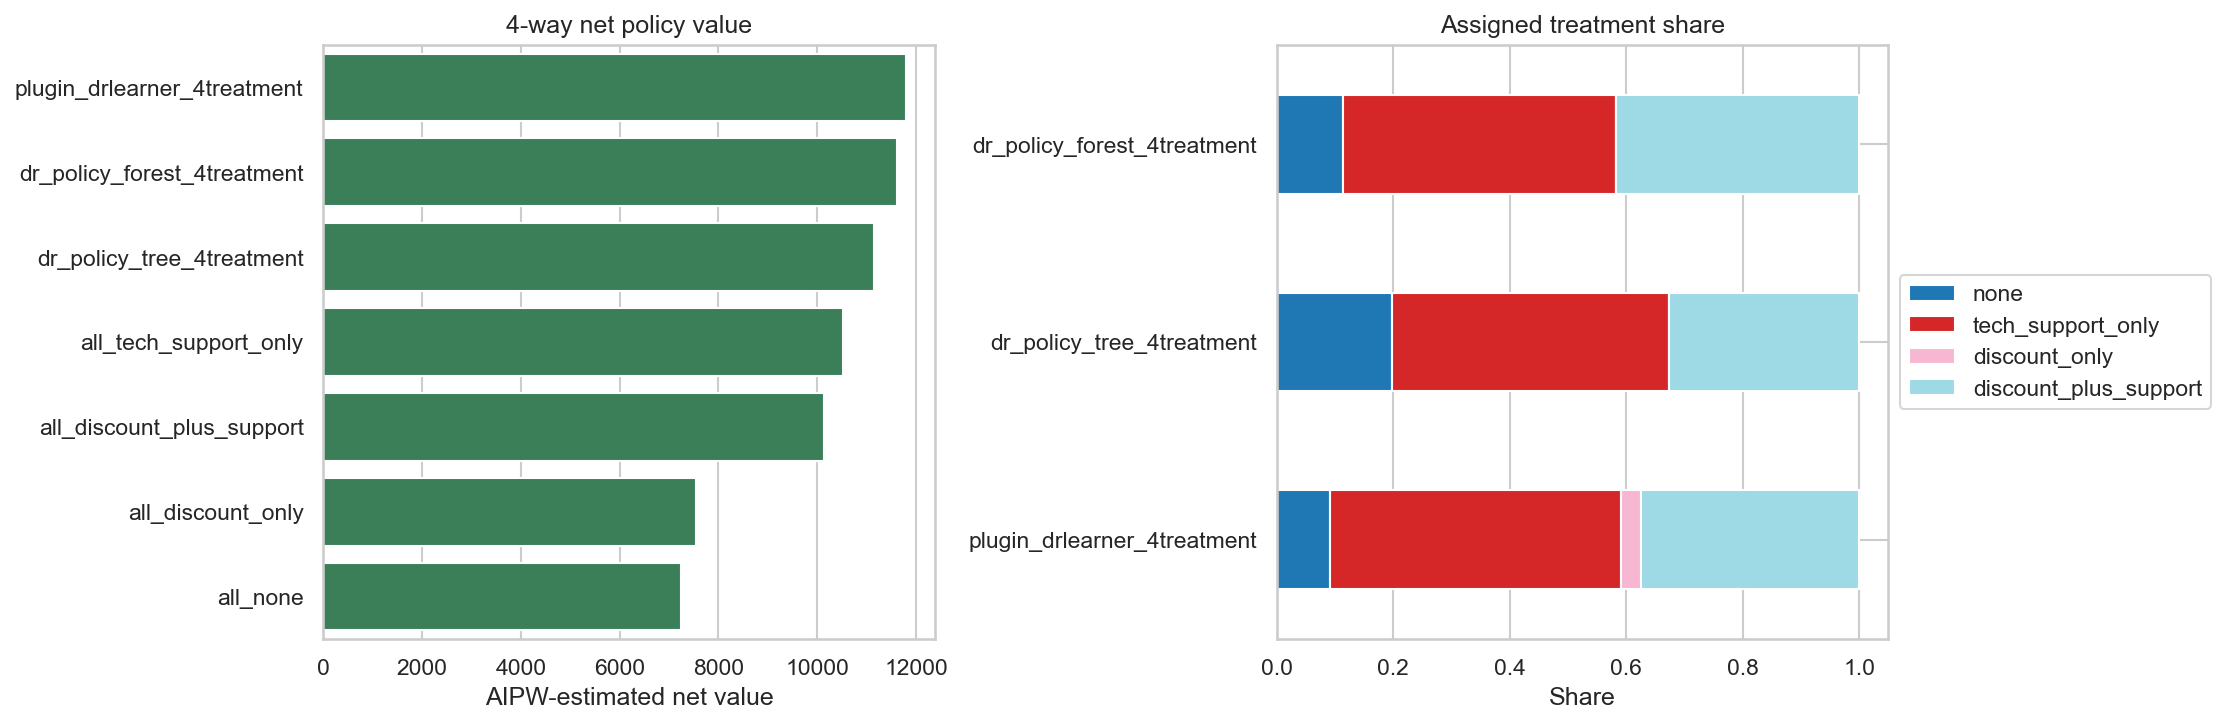
\includegraphics[width=0.95\textwidth]{fig07_policy_value.png}
\caption{(좌) 정책별 AIPW 순가치와 학습 포함 bootstrap 95\% CI. 세 학습 정책 모두 단일 처치 정책을 상회한다. (우) 학습 정책의 처치 배정 비중.}
\label{fig:value}
\end{figure}

세 학습 정책 모두 단일 처치 정책보다 높은 가치를 가진다(표~\ref{tab:value}, 그림~\ref{fig:value}). 고객별 타겟팅이 모두에게 같은 처치를 적용하는 것보다 효과적이라는 의미다. plug-in과 forest는 신뢰구간이 상당 부분 겹쳐 실질적 차이가 있다고 보기는 어렵다. 트리 정책은 해석 가능성을 유지하는 대신 성능을 일부 양보했다. \texttt{all\_discount\_plus\_support}가 \texttt{all\_tech\_support\_only}보다 낮은 이유는, 할인 비용이 고객 규모에 따라 커지도록 설정해 일부 고객에서 할인의 순수익이 비용을 상쇄하지 못했기 때문이다.

\textbf{Q4 요약.} 세 학습 정책 모두 최선의 단일 처치 정책보다 높은 순이익을 낸다(plug-in 기준 +12\%, 처치 없음 대비 +63\%). 타겟팅의 가치가 데이터로 확인된다.

% =================================================== Q5

\section{Q5. 예산이 제한되면 어떤 정책이 유리한가?}

앞의 Q4에서는 각 정책의 전체 평균 순이익을 비교했다. 그러나 실제 운영에서는 모든 고객에게 정책을 그대로 적용할 만큼 예산이 충분하지 않을 수 있다. 이 경우 중요한 질문은 ``어떤 정책의 평균 가치가 가장 높은가''가 아니라, ``같은 예산 안에서 어떤 정책이 더 많은 순이익을 만드는가''이다.

이를 비교하기 위해 비용 곡선(cost curve)을 사용한다. 각 정책이 처치를 배정한 고객에 대해 두 값을 계산한다.

\begin{itemize}[leftmargin=1.4em, itemsep=2pt]
  \item \textbf{예상 비용:} 해당 고객에게 그 처치를 제공하는 데 드는 비용
  \item \textbf{순이익 증가분:} 처치 없음 대비 AIPW 기준 순이익 증가분
\end{itemize}

그다음 고객을 \textbf{순이익 증가분 / 예상 비용} 비율이 높은 순서로 정렬한다. 즉, 같은 비용으로 더 큰 순이익을 낼 수 있는 고객부터 예산을 배정한다. 이 정렬 결과를 비용 곡선(그림~\ref{fig:cost})으로 시각화한다. 그림에서 x축은 누적 처치 비용, y축은 누적 순이익 증가분이며, 같은 x값에서 y값이 높을수록 같은 예산으로 더 높은 순이익을 내는 정책이다.

\begin{figure}[h]
\centering
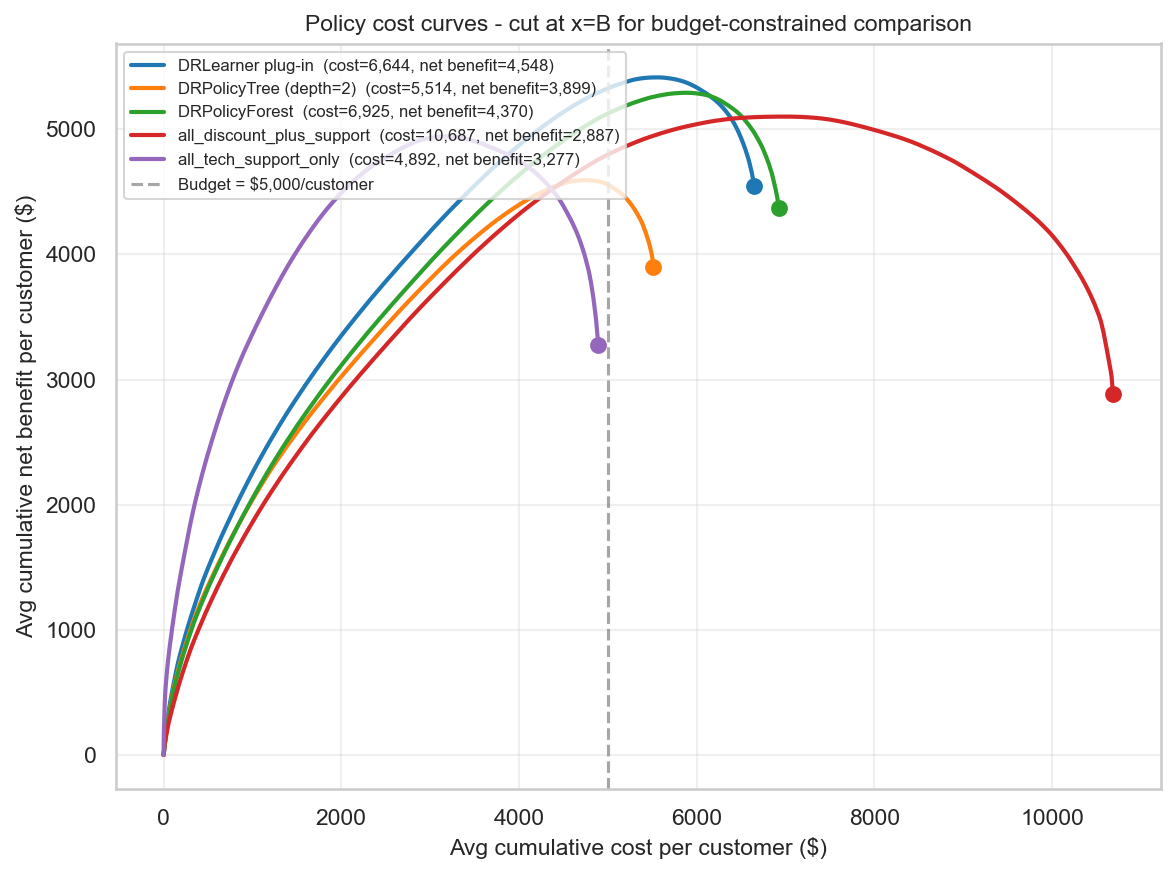
\includegraphics[width=0.85\textwidth]{fig08_cost_curve.png}
\caption{정책별 비용 곡선. 예산($x=B$)에서 y값이 높을수록 효율적이다. 학습 정책은 총 예산 \$3.9M 이상에서 전원 기술지원을 앞선다.}
\label{fig:cost}
\end{figure}


\textbf{왜 순이익만으로 정렬하지 않는가?} 예산이 제한되어 있을 때는 순이익의 절대 크기보다 비용 대비 효율이 중요하다. 예를 들어 A 고객사는 순이익 증가분이 \$10{,}000이지만 비용이 \$100{,}000이고, B 고객사는 순이익 증가분이 \$3{,}000이지만 비용이 \$5{,}000이라고 하자. 순이익만 보면 A가 더 좋아 보이지만, 예산이 \$10{,}000이라면 A는 처치할 수 없고 B는 처치할 수 있다. 따라서 예산 제약 하에서는 순이익이 큰 고객이 아니라, 비용 대비 순이익이 큰 고객부터 선택해야 한다.

\textbf{예산 규모에 따라 효율적인 정책이 다르다.}

\begin{itemize}[leftmargin=1.4em, itemsep=2pt]
  \item \textbf{소액 예산(\$3.9M 이하):} \texttt{all\_tech\_support\_only}가 가장 효율적이다. 기술지원 평균 비용이 낮아 순수익/비용 비율이 높은 고객부터 빠르게 처치할 수 있다.
  \item \textbf{중간 예산(\$3.9M\,$\sim$\,\$6M):} 학습 정책(plug-in, forest)이 앞선다. plug-in이 전원 기술지원을 추월하는 시점은 약 \textbf{\$3.9M}이다.
  \item \textbf{예산 전부 소진:} 학습 정책이 가장 효율적이고, \texttt{all\_discount\_plus\_support}가 효율이 가장 낮다(표~\ref{tab:costcurve}).
\end{itemize}

\FloatBarrier
\begin{table}[h]
\centering
\small
\caption{정책별 총 비용 · 총 순이익 (test set 1{,}000곳 누적 합계)}
\label{tab:costcurve}
\begin{tabular}{lrr}
\toprule
정책 & 총 비용 & 총 순이익 \\
\midrule
DRLearner plug-in & \$6.6M & \$4.6M \\
DRPolicyForest & \$6.9M & \$4.4M \\
DRPolicyTree (depth=2) & \$5.5M & \$3.9M \\
all\_tech\_support\_only & \$4.9M & \$3.3M \\
all\_discount\_plus\_support & \$10.7M & \$2.9M \\
\bottomrule
\end{tabular}
\end{table}

\texttt{all\_discount\_plus\_support}는 총 \$10.7M을 소진해도 순이익이 \$2.9M에 그쳐 효율이 가장 낮다. 할인 비용이 고객 규모에 따라 커지도록 설정해 일부 고객에서 순수익이 비용을 상쇄하지 못했기 때문이다.

\textbf{Q5 요약.} ``어떤 정책이 최선인가''는 예산에 의존한다. 예산이 적으면 저비용 단일 처치가, 예산이 충분하면 타겟팅 정책이 유리하다. 비용 곡선은 예산을 고려한 의사결정에 직접 활용할 수 있는 도구다.

% =================================================== 결론
\section{결론 및 제언}

약 2{,}000곳의 관찰 데이터에서, 비용을 반영한 순이익을 기준으로 네 가지 프로모션의 고객별 최적 배정을 학습했다. 처치 효과의 이질성을 진단(Q1)하고 인과 식별 가정을 점검(Q2)한 뒤, 세 가지 정책을 학습(Q3)하고 학습/평가 데이터를 분리해 doubly robust(AIPW) 기준으로 가치를 비교(Q4)했으며, 예산 제약 하의 효율(Q5)까지 평가했다.

\textbf{비즈니스 제언.}
\begin{enumerate}[leftmargin=1.6em, itemsep=2pt]
  \item \textbf{고객별 타겟팅이 단일 정책보다 효과적이다.} 최선의 단일 처치 대비 약 12\%, 처치 없음 대비 약 63\% 높은 순이익을 낸다.
  \item \textbf{처치 배정의 핵심 신호는 고객 규모와 직원 수다.} 규모가 큰 고객에게는 기술지원+할인, 그 외에는 주로 기술지원이 적합하다. 기대 순이익이 낮은 일부는 처치 없음이 유리하다.
  \item \textbf{예산 규모에 따라 최적 정책이 달라진다.} 총 예산 \$3.9M 이하라면 전원 기술지원이, 그 이상이라면 학습 정책이 더 높은 순이익을 낸다.
  \item \textbf{성능과 해석 가능성 사이에서 선택이 필요하다.} 성능 최우선이면 plug-in/forest가, 이해관계자 설명과 운영 안정성이 중요하면 depth=2 트리 정책이 적합하다.
\end{enumerate}

\textbf{한계와 다음 단계.}
\begin{itemize}[leftmargin=1.4em, itemsep=2pt]
  \item 본 분석은 관찰 데이터 기반의 오프라인 추정이다. Unconfoundedness는 검정할 수 없는 가정이므로, 관측되지 않은 요인이 처치 배정과 성과에 동시에 영향을 미쳤다면 정책 가치가 편향될 수 있다.
  \item 비용은 실제 집행 비용이 아니라 시뮬레이션 값이다. 실제 할인 비용과 기술지원 운영 비용이 확보되면 순이익과 예산 기준의 결론이 달라질 수 있다.
  \item 학습 포함 bootstrap 신뢰구간에서 상위 정책 간 구간이 일부 겹친다. 따라서 현재 결과는 정책 간 우열을 확정한다기보다, 타겟팅 정책이 단일 정책보다 유망하다는 근거로 해석하는 것이 적절하다.
  \item 실제 적용 이후에는 A/B 테스트가 가능하면 직접 검증하고, 어렵다면 AIPW 기반 사후평가와 성과 모니터링을 통해 정책을 주기적으로 점검해야 한다.
\end{itemize}

% =================================================== 참고
\section*{\sffamily\color{brand} 참고 자료}
\small
\begin{itemize}[leftmargin=1.4em, itemsep=2pt]
  \item Athey, S., \& Wager, S. (2021). \emph{Policy Learning with Observational Data}. Econometrica. \href{https://arxiv.org/abs/1702.02896}{arxiv.org/abs/1702.02896}
  \item Sun, L., Du, X., Wager, S., et al. (2021). \emph{Treatment Allocation under Uncertain Costs}. \href{https://arxiv.org/abs/2103.11066}{arxiv.org/abs/2103.11066}
  \item Imai, K., \& Li, M. L. (2019). \emph{Experimental Evaluation of Individualized Treatment Rules}. \href{https://arxiv.org/pdf/1905.05389.pdf}{arxiv.org/pdf/1905.05389}
  \item Stanford ML+CI Tutorial --- \emph{Policy Learning I (Binary Treatment)}.
  \item Microsoft SynapseML. \emph{Quickstart - Measure Causal Effects}. \href{https://microsoft.github.io/SynapseML/docs/Explore%20Algorithms/Causal%20Inference/Quickstart%20-%20Measure%20Causal%20Effects/}{공개 샘플 데이터: multi-attribution sample CSV}
\end{itemize}

\vspace{1em}
{\color{rulegray}\hrule}
\vspace{4pt}
{\footnotesize\color{ink} \textbf{조해창} · 데이터 분석 포트폴리오 · 코드와 재현 가능한 분석: \href{https://github.com/Funbucket/Promotion-Targeting-with-Policy-Learning}{GitHub Repository}.}

\end{document}
